% !TeX root = ../main.tex
\chapter{System Architecture Design}
\label{chap:system_architecture}

\section{Introduction}

In this chapter, we delve deeper into the system architecture design. As illustrated in Figure \ref{fig:e2e-architecture}, the proposed solution is structured into distinct, modular tiers, forming an End-to-End Streaming Architecture.

The system relies on the following core layers:
\begin{itemize}
\item \textbf{Source Systems Layer:} This tier acts as the primary origin of truth. For the scope of this study, it comprises a high-performance simulation environment that generates all necessary operational and physical telemetry variables for subsequent analytics. In a prospective industrial deployment, this layer can be seamlessly extended to incorporate physical, production-grade autonomous mobile robots.
\item \textbf{Broker MQTT Layer:} Serving as the initial edge gateway, this layer receives live telemetry payloads published directly by the source systems. While future iterations of the architecture might bypass this boundary—routing data directly through the central event streaming bus—deploying an independent MQTT broker establishes a robust and lightweight communication bridge tailored for IoT edge devices and complies with the requirements of the VDA50505 protocol.
\item \textbf{Event Streaming Layer:} Functioning as the central nervous system of the application, this layer acts as a distributed event bus. It decouples the data emitters from the compute engines, guaranteeing reliable, low-latency message buffering and high-throughput streaming across the pipeline.
\item \textbf{Stream \& Processing Layer:} Dedicated to continuous stream processing, this layer performs real-time computations and data transformation. It is architected to efficiently handle and process massive volumes of high-frequency data streams.
\item \textbf{Data Lakehouse Layer:} Operating as the persistence backbone, this layer stores the historical telemetry required for downstream machine learning analytics. By adopting a Data Lakehouse paradigm, the system combines cost-effective object storage with DBMS-like ACID transactions. Furthermore, it implements the \textit{Medallion Architecture} (Bronze, Silver, and Gold tiers), preserving raw immutable ingestion data to ensure full reprocessing flexibility over time.
\item \textbf{Machine Learning Layer:} This analytical module fulfills the primary objective of the research: real-time anomaly detection through advanced machine learning models consuming refined features from the data lakehouse.
\item \textbf{Observability Layer:} Once operational metrics and diagnostic outputs are consolidated in the Gold layer, this tier presents actionable insights to operators through comprehensive visualization dashboards, enabling real-time monitoring of system health and robot anomalies.
\end{itemize}
\begin{figure}[ht]
  \centering
  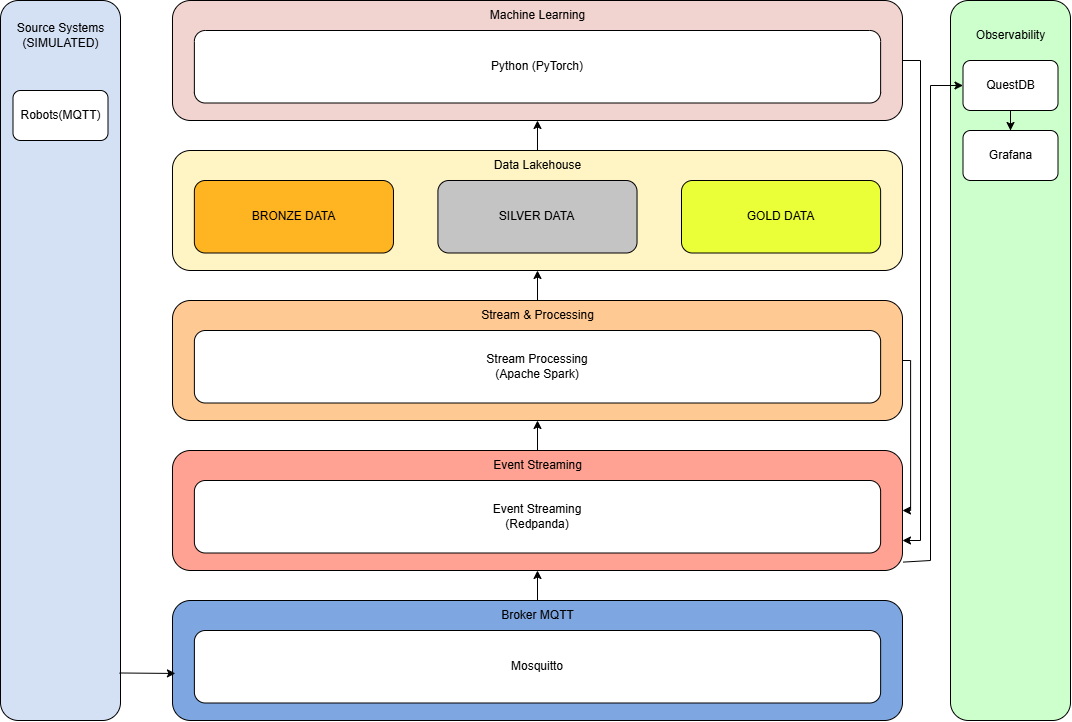
\includegraphics[width=.85\linewidth]{TFGArquitectura.drawio.png}
  \caption{Arquitechture schema from the E2E anomaly detection system.}
  \label{fig:e2e-architecture}
\end{figure}
\section{General Architectural Decisions}

In addition to the component-specific design decisions presented in the following sections, several cross-cutting architectural principles were established to guide the development of the entire platform.

\subsection{Containerized Microservice Architecture}

The complete platform was designed following a containerized microservice approach. Each functional layer of the architecture is deployed as an independent Docker container, including the source systems, messaging infrastructure, stream processing services, data storage components, and machine learning modules.

This modular design provides several advantages. First, it promotes loose coupling between system components, allowing individual services to be developed, tested, and maintained independently. Second, it simplifies system scalability, since each component can be replicated or upgraded without affecting the rest of the platform. Finally, it increases the long-term maintainability of the solution, as individual modules may be replaced by alternative implementations provided that the communication interfaces remain unchanged. Consequently, the architecture is centered on well-defined interfaces rather than on specific software implementations, facilitating future evolution of the platform.

\subsection{Interface-Oriented Design}

To maximize interoperability and future extensibility, communication between architectural layers is performed through standardized interfaces and message formats. This design principle ensures that a component can be replaced without requiring major modifications in the remaining layers. For example, the simulated AGV fleet used during development could be replaced by a real fleet management system, while preserving the same MQTT and VDA 5050 communication contracts. As a result, the architecture remains independent of specific hardware vendors or software providers.

\subsection{Continuous Integration and Version Control}

The development process follows modern software engineering practices based on distributed version control and continuous integration principles. Git was adopted as the central version control system, enabling traceability of architectural decisions, source code modifications, configuration changes, and experimental results throughout the project lifecycle. In addition, the containerized nature of the platform facilitates the implementation of future Continuous Integration and Continuous Deployment (CI/CD) pipelines, allowing automatic validation, testing, and deployment of updated system components.

\subsection{Event-Driven Architecture} An event-driven architecture was adopted as the communication paradigm for the entire platform. Rather than relying on direct point-to-point interactions between services, all components communicate through an intermediate event streaming layer. This approach significantly reduces coupling between producers and consumers, allowing individual services to evolve independently without affecting other parts of the system. Additionally, new services can be integrated into the platform with minimal effort by subscribing to the existing event streams. The event streaming layer acts as the system's central source of truth, providing a unified and consistent mechanism for distributing telemetry, operational events, and analytical results across the architecture. This design improves scalability, extensibility, and maintainability while facilitating the integration of future data processing and monitoring capabilities.

\section{Source Systems Layer}
In designing the data ingestion pipeline, a preliminary study was conducted to determine the optimal source of truth for the system. At first, the possibility of utilizing a physical Autonomous Mobile Robot (AMR) in real time was evaluated. However, this approach was discarded for the training phase due to two primary constraints: first, a single available unit is insufficient to represent a fleet-scale source system; second, the physical hardware lacked the specific internal telemetry sensors required for comprehensive anomaly detection analytics.

As a second approach, a search was conducted for publicly available industrial datasets containing multi-variable telemetry from AGVs and AMRs. While several sources were identified, none provided the precise combination of electrical, mechanical, and thermal variables necessary for the anomaly detection module.

Given the limitations of both physical deployments and existing public datasets, the decision was made to implement a high-performance simulation framework capable of emulating an entire fleet of AGVs deterministically. Since the chosen simulation environment, built upon the open-source repository \texttt{bekirbostanci/vda5050\_vehicle\_simulator} \cite{bostanciVda5050},, did not natively incorporate deep physical powertrain dynamics, it was adapted to model core electromechanical and thermal variables. To ensure seamless integration with downstream data consumers, the messages published by the simulated robots strictly adhere to the \textbf{VDA 5050} \cite{vda5050standard} interoperability standard, extended to include custom telemetry payloads.

The following JSON payload illustrates the structure of the telemetry and state messages emitted by the adapted source systems:

\begin{lstlisting}[language=json, caption={Example VDA 5050 telemetry message}, label={lst:vda5050-telemetry}, basicstyle=\ttfamily\small, breaklines=true]
{
  "actionStates": [],
  "agvPosition": {
    "mapId": "messe_f1",
    "positionInitialized": false,
    "theta": 0,
    "x": -0.26424313,
    "y": -1.4748409
  },
  "batteryState": {
    "batteryCharge": 99.8,
    "batteryHealth": 100,
    "batteryVoltage": 24.023438,
    "charging": false
  },
  "driving": false,
  "edgeStates": [],
  "errors": "[]",
  "headerId": 20,
  "information": "[{\"infoDescription\":\"Dynamic powertrain telemetry\",\"infoLevel\":\"INFO\",\"infoReferences\":[{\"referenceKey\":\"motor_current\",\"referenceValue\":\"0.45\"},{\"referenceKey\":\"motor_voltage\",\"referenceValue\":\"24.02\"},{\"referenceKey\":\"motor_temp\",\"referenceValue\":\"24.73\"},{\"referenceKey\":\"vibration_rms\",\"referenceValue\":\"0.011\"},{\"referenceKey\":\"motor_speed_rad_s\",\"referenceValue\":\"0.00\"},{\"referenceKey\":\"motor_torque_nm\",\"referenceValue\":\"0.000\"},{\"referenceKey\":\"back_emf_v\",\"referenceValue\":\"0.00\"},{\"referenceKey\":\"wheel_slip\",\"referenceValue\":\"0.0042\"},{\"referenceKey\":\"motor_power_w\",\"referenceValue\":\"0.4\"},{\"referenceKey\":\"battery_current_a\",\"referenceValue\":\"0.43\"},{\"referenceKey\":\"battery_soc_pct\",\"referenceValue\":\"99.80\"},{\"referenceKey\":\"battery_health_pct\",\"referenceValue\":\"100\"},{\"referenceKey\":\"battery_temp_c\",\"referenceValue\":\"21.9\"},{\"referenceKey\":\"fault_active\",\"referenceValue\":\"false\"},{\"referenceKey\":\"fault_types\",\"referenceValue\":\"\"}],\"infoType\":\"motor_telemetry\"}]",
  "lastNodeId": "",
  "lastNodeSequenceId": 0,
  "loads": [],
  "manufacturer": "rikeb",
  "nodeStates": [],
  "operatingMode": "AUTOMATIC",
  "orderId": "",
  "orderUpdateId": 0,
  "safetyState": {
    "eStop": "NONE",
    "fieldViolation": false
  },
  "serialNumber": "t13",
  "timestamp": "2026-10-14T09:25:18.783Z",
  "velocity": {
    "omega": 0,
    "vx": 0,
    "vy": 0
  },
  "version": "2.0.0"
}
\end{lstlisting}

\section{MQTT Broker Layer} 
The adoption of the VDA 5050 communication standard directly influenced the design of the messaging layer. Since VDA 5050 defines MQTT as the underlying communication protocol between fleet management systems and AGVs, the incorporation of an MQTT broker became a fundamental architectural requirement. 

The broker layer acts as an intermediary between telemetry producers and data consumers, enabling asynchronous communication and decoupling the different system components. This approach allows producers and consumers to evolve independently while maintaining interoperability through standardized message exchanges. 

Several MQTT broker implementations were evaluated during the architectural design phase. Eclipse Mosquitto was ultimately selected due to its maturity, open-source licensing model, low resource consumption, Docker compatibility, and widespread adoption within Industrial Internet of Things (IIoT) environments. 

Furthermore, the publish/subscribe communication model facilitates horizontal scalability and simplifies the integration of future services. New consumers can subscribe to existing telemetry streams without requiring modifications to the source systems, making the architecture more extensible and maintainable.

\section{Summary}
